
\section{Discussion}
\subsection{summer winds}
Three main patterns of upwelling favorable winds have been
described. Two of them, SSW and SSE winds
(Fig~\ref{fig:windsreconfig}c and d), dominate while the SW wind
(Fig~\ref{fig:windsreconfig}a) occurs more sporadically. The
period under study, July 1999 through to May 2001, was
characterized by the absence of a clear seasonal wind signal with
upwelling and downwelling winds distributed year-around. Similar
results were obtained by \nocite{nogueira98}\markcite{{\it
Nogueira }[1998]}, who found that only 20\% the variability in
daily Ekman transport off Cape Finisterre over 9 years was
associated with the seasonal cycle, while 70\% concentrated at
frequencies $<$30 days. This is in contrast to other eastern
upwelling areas like California. Comparing our data with those of
\nocite{kosro91}\markcite{{\it Kosro et al.}[1991]} we observe
that although cycles of upwelling-winds/relaxation take place in
both regions, Galicia is more variable in wind speed and direction
and persistence during the two years studied. Much of the summer
variability is related to the passages of anticyclones moving
northeastward over the bay of Biscay. The time scale of $14\pm 2$
days determined here is close to that ($T=15\pm 5$ days) from
harmonic analysis of 9 years of daily upwelling indices off Cape
Finisterre during the upwelling season
\nocite{Nogueira97}\markcite{[{\it Nogueira et al., }1997]}.

The alternation of the above wind fields forces different
responses in the system favoring either north or west coast
upwelling. Summer 1999 experienced winds favorable to north coast
upwelling and Cape Finisterre filament development while summer
2000 was more typified by west coast upwelling. Both years
experienced highly variable winds that did not persist long enough
for upwelling filaments to develop on the west coast. The
strongest development of west coast filaments in recent years
occurred in 1998, when west coast upwelling-favorable winds lasted
from June to early August,with few interruptions. These sustained
upwelling favorable winds maintained a sharp upwelling front that
allowed the development and growth of the west coast instabilities
into upwelling filaments.

Much has been hypothesized about the generation of upwelling
filaments.  \nocite{Roed99, Haynes93} \markcite{{\it Roed and
Shi,} [1999] and {\it Haynes et al.,} [1993]} reported a clear
link between bottom topography and filament formation in the
Galician region on the basis of models and observations,
respectively. However, in the case presented here, the Cape
Finisterre filament clearly is dependent on particular wind
conditions for its development. The mere presence of upwelling at
Finisterre is not sufficient. Although small scale instabilities
sometimes develop off the Cape (see Figs~\ref{fig:windssst2123}b,d
and \ref{fig:windssst95}a), it requires a well developed north
coast upwelling for them to grow into a full sized filament. At
these times the wind field is like that of
Fig~\ref{fig:windsreconfig}a and the filament extends offshore
along the line of maximum wind curl identified in mode 2 in
Fig~\ref{fig:windseofseasonal}.
\begin{figure}
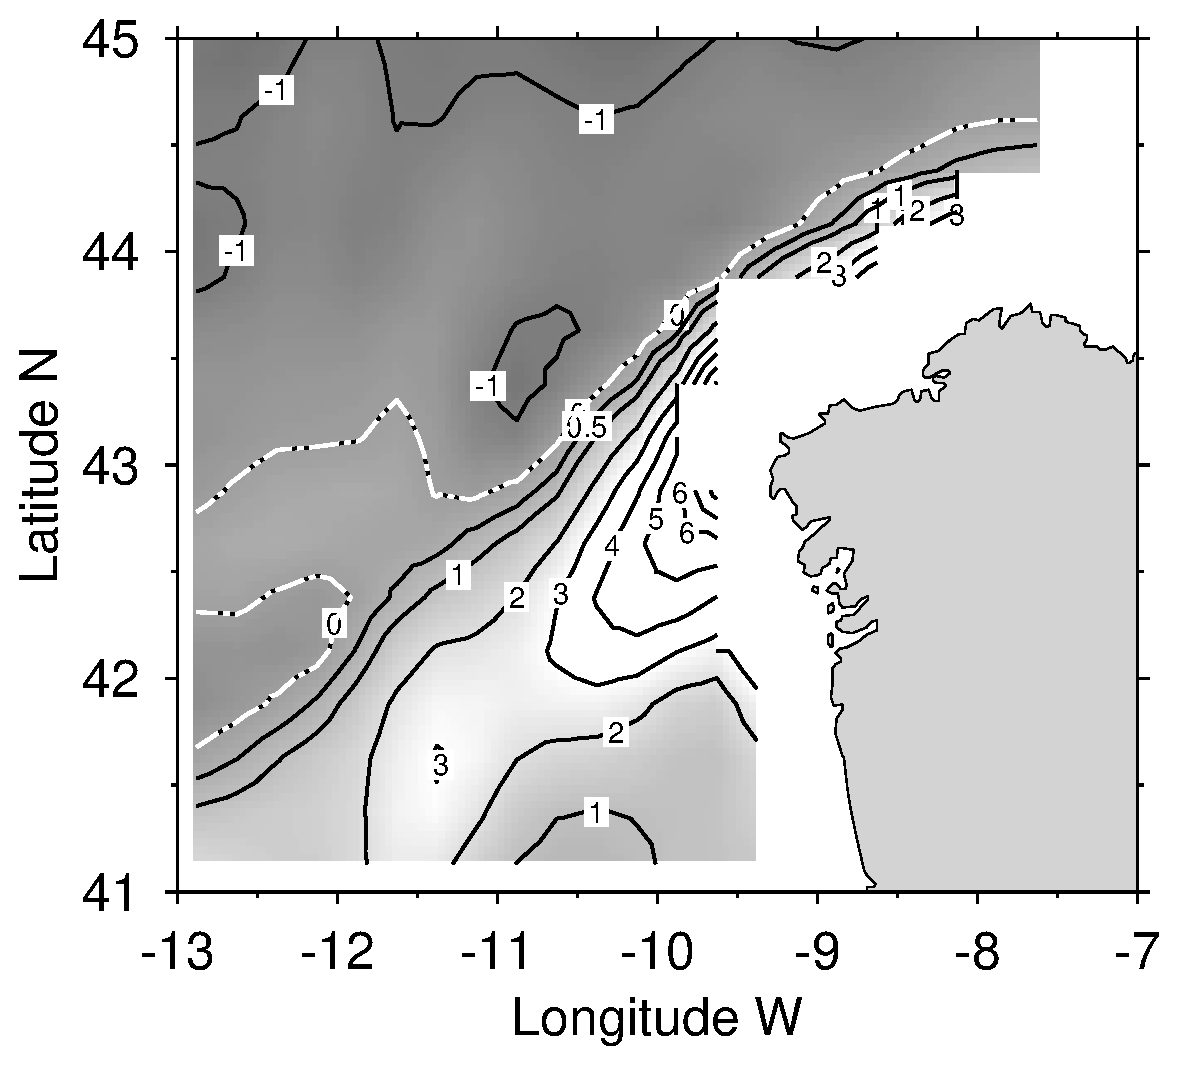
\includegraphics[height=8cm]{ekman_pum_1999723}%ekman_pum_1999723}
\caption{Vertical Ekman pumping velocities on 22 July 1999 in
m/day, positive upwards.} \label{fig:ekman}
\end{figure}

This maximum wind curl produces upwelling velocities given by
\(w=k\cdot(\nabla \times \frac{\tau}{f\rho} )\), where $k,\tau,f$
and $\rho$ are vertical unit vector, wind stress, Coriolis
parameter and density of water. This Ekman pumping is caused
solely by the divergent Ekman fluxes in the presence of spatially
variable wind and is unrelated to the coastal upwelling.  An
example is shown in Fig~\ref{fig:ekman} for measured winds on 22
July 1999 corresponding to a wind field similar to
Fig~\ref{fig:windsreconfig}a. Positive Ekman pumping velocities
indicative of upwelling can be seen south of the maximum wind curl
northern limit in Fig~\ref{fig:windseofseasonal}b and towards the
west coast. Maximum vertical velocities coincided with the axis of
maximum curl and decreased from 6m/day near Cape Finisterre to
1m/day farthest offshore. Similar calculations on a day in March
2000 yielded a similar pattern except vertical velocities were
smaller by a factor of 2 and decreased rapidly on the west coast.

Winds in June 1995 (Figs~\ref{fig:windsslp}a and b) were stronger
than in March 2000 because of the presence of the summer Iberian
low. We conclude summer occurrences of this wind pattern lead to
upwelling velocities of 5-6m/day off Cape Finisterre. These are
smaller than the ones reported by \nocite{munchow00}\markcite{{\it
M\"{u}nchow }[2000]} off Point Conception. Their finer sampling
covered a much smaller area which defined a maxima wind curl ridge
80km long and 10km wide. In our case, the ridge extends 320km in
length and 90km in width and vertical velocities are likely to
reach higher values nearer to the shore at Cape Finisterre.
\begin{figure}
\includegraphics[height=8cm]{wind_july9977march00320}
\caption{Example of measured winds from the offshore buoys on 7
July 1999 (black) and 20 March 2000 (red).} \label{fig:rev}
\end{figure}

Evidences of reverse wind flow in the lee of Cape Finisterre
during the summer upwelling regime can be found in the offshore
buoys wind data shown in Fig~\ref{fig:rev} for 7 July 1999 (black)
and 20 March 2000 (red). Wind conditions are very similar on both
days in the north coast (Bares buoys; no data were recorded at
Villano-Sisargas in March 2000) while measured winds at Silleiro
flowed nearly in opposite directions; the July example flowing
onshore is indicative of strong flow separation at the cape.
Similar situations were common throughout March 2000 and after 14
June 1999, the main difference being the presence of cold upwelled
water around Cape Finisterre during the 1999 examples.
\nocite{munchow00}\markcite{{\it M\"{u}nchow }[2000]} describes
identical conditions whereby similar wind fields produced stronger
flow separation at Point Conception in the presence of upwelling.
They argued that the lower sea surface temperatures enhanced the
vertical stability of the lower atmosphere and that it could
probably be related with the temperature inversion found at the
top of the marine layer. Like in \nocite{Enriquez95}\markcite{{\it
Enriquez and Friehe }[1995]}, the marine layer behaves as a
supercritical flow and separates from the coast causing the wind
curl and associated Ekman pumping velocities. Hence, there are
evidences that the NCUP strengthen both near the coast and after
the start of the coastal upwelling generating larger wind curl and
associated Ekman pumping velocities increasing shorewards. The
positive wind curl would cause a poleward alongshore pressure
gradient as indicated by model studies of \citet{Wang97}.

\nocite{munchow00}\markcite{{\it M\"{u}nchow }[2000]} showed that
a similar wind curl influenced the vertical water structure to
cause doming of the isopycnals.  A similar local effect on the
shelf circulation may be expected around Cape Finisterre. The
systematically weaker southward velocities observed at the west
coast buoy (W) compared to the Finisterre buoy (F) are consistent
with such a cyclonic tendency but we presently have no
hydrographic evidence to verify it. Coastal topographic features,
in particular capes, also have a significant impact on the
alongshore variability of the upwelling flow field
\citep{Crepon84,Dale01,Rosenfeld94}. Intensified nonlinear effects
accompany the acceleration of the flow around the capes that
influences the local alongshore pressure balance. During upwelling
favorable wind, with southward wind-driven currents, lower
pressure off the cape and higher pressure downstream of it
generate a northward pressure gradient south of the cape which is
consistent with the weaker velocities found at buoy W. Doming
could also explain the persistence of the Finisterre filament
following cessation of favorable wind patterns, e.g. after 24 June
(Fig~\ref{fig:windssst2123}).
\subsection{winter winds}

Winter winds in general showed larger variability than summer
winds during both a ``typical'' (2000-2001) and ''atypical''
(1999-2000) seasonal years. Downwelling wind patterns were drawn
from CEOF analysis during both the 1999-2000 and winter 2001
analysis. E,EN and N were predominant during both winters reaching
speeds in the range 15-20\vel, higher than the 10-15\vel\, range
that characterized summer winds. However their persistence was far
less than during summer, 4-6 days compare to the 12 days found for
summers 1999 and 2000. Winters 2000 and 2001 both saw the NCUP
wind field predominate during sustained periods in March and
February respectively. Its effect in the SST field showed the
disappearance of the warm SST anomaly linked to the poleward flow
only in the north coast, but not in the west coast. Similar
conclusions were drawn from the 2000 winter current record.


Winter currents were only available during winter 2000, which
overall was ``atypical'', but it showed some characteristics that
might be common to more ``normal'' years. Poleward flow was more
consistent in the west coast, in agreement with the JEBAR forcing,
although larger velocities were measured in the northern buoy. At
this location, the wind had a larger effect and currents
alternated from equatorward to poleward flow, although mean
currents during the entire record corresponded to weak poleward
flow of 3\velc. The meridional SST temperature gradient follows a
marked seasonality with a maximum of -0.5\deg $ /100 km^{-1}$
around March-April and a minimum of -0.15\deg $ /100 km^{-1}$ in
August when estimated from weekly averages of SST images for a
transect at -10\deg W from 41\deg to 43\deg N. This translates
into density gradients of 0.1ppt/100km and 0.04ppt/100km. The
winter gradient could drive a 10\velc\, poleward current through
JEBAR forcing. Very often a localized maximum of twice the large
scale gradient can be seen at 42.5\deg N.

It is difficult to define transitional regimes, non-upwelling to
upwelling and vice versa in terms of the wind forcing. Attention
must be paid as to when do they take place. While the meridional
gradient is present, (nearly until July) upwelling winds do not
fully set up upwelling; sustained winds that should have developed
filaments they do not like in April-May 2001. Although upwelling
did develop, one week without northerly winds and the upwelling
band disappeared.

\section{Conclusions}
Our study of the QuikSCAT and in situ wind fields in the Galician
upwelling region around Cape Finisterre has shown:
\begin{enumerate}
  \item    The wind field is far from homogeneous in the region so that
wind observations at a single point, coastal or offshore, will not
necessarily be representative of coastal conditions over any
significant distance.

  \item   The wind field's long-term mean summer and winter patterns are
not necessarily representative of particular years when, as we
have seen, summer-like patterns may dominate in winter also.

  \item   Similar Wind Modes were obtained in all CEOF analysis, of both
satellite derived and \emph{in situ} buoy measurements, and of
different length and seasonal period.

  \item   Summer time wind fields have a small number of dominant
patterns, discernible in complex empirical orthogonal analysis,
that are responsible for the typical distributions of upwelling in
and off the Galician coast.

  \item   One pattern produces north coast, but no west coast,
upwelling. In years when this pattern dominates, the Cape
Finisterre filament is strong but no others develop. The filament
is partly supplied by cold water from the north coast but also,
importantly, by local open ocean upwelling produced by the wind
stress curl, which extends in a maximum SW from the cape.

  \item   Another pattern produces west coast upwelling, but no
north coast upwelling.  When this pattern persists, west coast
filaments develop at favored locations other than Finisterre and
may extend up to 200km offshore.

  \item   These patterns may alternate producing brief episodes or north
or west coast upwelling with little filament development, or a
combined pattern may occur that produces weak upwelling on both
coasts with a localized maximum at Finisterre, where the wind lies
parallel to the coast.

  \item   Winter time wind patterns show strong similarities to those of
summer, symptomatic of frequent short occurrences of winter
upwelling during our study years.

  \item   The onset of the winter poleward flow regime as indicated by
presence of the warm water anomaly along the continental slope is
delayed after the cessation of summer upwelling winds.  Likewise
the spring onset of upwelling lags significantly the commencement
of favorable winds, though subsequent upwelling events respond
rapidly to wind changes.

  \item   North coast currents were more variable in all records
  and showed the largest velocities during both upwelling and
  non-upwelling regimes.
\end{enumerate}


Although there have been various significant efforts to observe
facets of the Galician or Iberian upwelling over the years e.g.
recently MORENA, OMEX II, there has never been a systematic effort
to monitor its year-round physical development with simultaneous
hydrographic, current and meteorological observations on the scale
of the California Current programs like CUEA, CODE, . The
gradualist approach, while it has illuminated many aspects of the
system, has left many basic questions like the 3-d structure, the
spin up and spin down of upwelling, the importance of alongshore
propagating upwelling signals, unanswered.
